\documentclass[tikz,border=10pt]{standalone}
\usepackage{amsmath}
\usepackage{tikz}
\usetikzlibrary{arrows.meta, positioning, angles, quotes, decorations.markings, calc}

\begin{document}

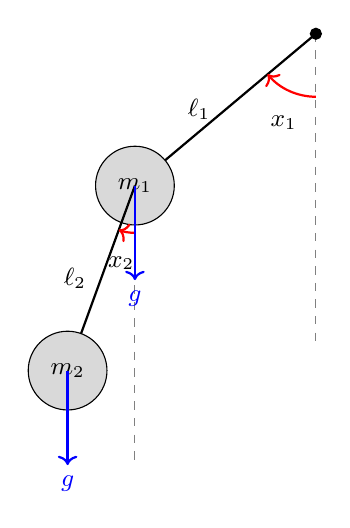
\begin{tikzpicture}[
  mass/.style = {circle, draw, fill=gray!30, minimum size=1cm},
  string/.style = {thick},
  anglemark/.style = {draw, ->, thick, red},
  force/.style = {->, thick, blue},
  arrow/.style = {thick, -{Latex[width=2mm]}},
  every node/.style = {font=\small}
]

% Parameters
\def\Lone{3}
\def\Ltwo{2.5}
\def\thetaone{40}  % angle of first pendulum (deg)
\def\thetatwo{30}  % angle of second pendulum (deg)

% Coordinates
\coordinate (pivot) at (0,0);
\coordinate (m1) at ($(pivot) + (\thetaone:-\Lone)$);
\coordinate (m2) at ($(m1) + (\thetaone + \thetatwo:-\Ltwo)$);

% Draw vertical dashed lines (for both pendulums)
\draw[dashed, gray] (pivot) -- ++(270:\Lone+1);
\draw[dashed, gray] (m1) -- ++(270:\Ltwo+1);

% First pendulum
\draw[string] (pivot) -- (m1);
\node[mass] at (m1) {$m_1$};
\filldraw[black] (pivot) circle (2pt);

% Second pendulum
\draw[string] (m1) -- (m2);
\node[mass] at (m2) {$m_2$};

% Angle x1 (from vertical to first rod)
\draw[anglemark] (pivot) ++(270:0.8) arc[start angle=270, end angle={270 - \thetaone - 10}, radius=0.8];
\node at ($(pivot)+({270 - 0.5*\thetaone}:1.2)$) {$x_1$};

% Angle x2 (from vertical to second rod)
\draw[anglemark] (m1) ++(270:0.6) arc[start angle=270, end angle={280 - \thetatwo}, radius=0.6];
\node at ($(m1)+({275 - 0.5*\thetatwo}:1.0)$) {$x_2$};

% Gravity vectors
\draw[force] (m1) -- ++(0,-1.2) node[below] {$g$};
\draw[force] (m2) -- ++(0,-1.2) node[below] {$g$};

% Length labels
\path (pivot) -- node[midway, left=2pt] {$\ell_1$} (m1);
\path (m1) -- node[midway, left=2pt] {$\ell_2$} (m2);

\end{tikzpicture}

\end{document}
